% 2013 年北京卷理科第 17 题：三棱柱 ABC-A1B1C1。
% 来源 PDF：普通高考/2013/2013北京理.pdf，第 2 页（印面 788）左栏。
% AA1C1C 是边长为 4 的正方形，平面 ABC⊥平面 AA1C1C，AB=3，BC=5。
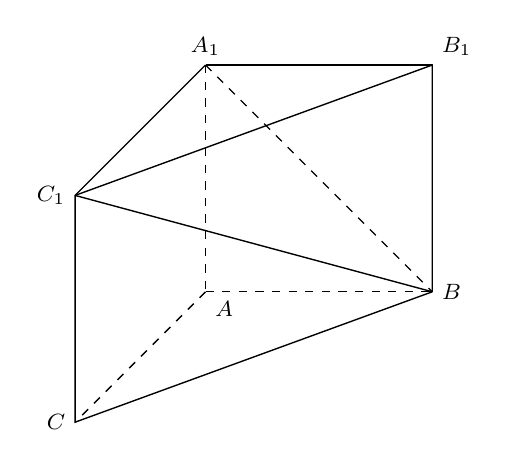
\begin{tikzpicture}[font=\footnotesize, line width=0.5pt, scale=0.72]
  % 正方形侧面 AA1C1C（平行四边形画法）：A1 在上，C1 在左上，A 在下，C 在左下
  \coordinate (A1) at (0,0);
  \coordinate (C1) at (-2.3,-2.3);
  \coordinate (A)  at (0,-4.0);
  \coordinate (C)  at (-2.3,-6.3);
  % AB 垂直于侧面，B 在右前方
  \coordinate (B)  at (4.0,-4.0);
  \coordinate (B1) at (4.0,0);
  % 可见棱
  \draw (A1) -- (C1) -- (C) -- (B);
  \draw (C1) -- (B1) -- (B);
  \draw (A1) -- (B1);
  % 被遮挡的棱
  \draw[dashed] (A1) -- (A);
  \draw[dashed] (A) -- (C);
  \draw[dashed] (A) -- (B);
  % 辅助线 A1B、C1B
  \draw[dashed] (A1) -- (B);
  \draw (C1) -- (B);
  % 顶点标签
  \node[above] at (A1) {$A_1$};
  \node[left] at (C1) {$C_1$};
  \node[above right] at (B1) {$B_1$};
  \node[below right] at (A) {$A$};
  \node[right] at (B) {$B$};
  \node[left] at (C) {$C$};
\end{tikzpicture}
